\chapter{Data Visualization and Communication}
\label{ch:visualization}
\chapterguide
  {You should understand distributions, grouped comparisons, outliers, and relationships.}
  {choose charts by analytical purpose; map variables to visual encodings; and write interpretations that do not overclaim.}

\section{Choose the chart from the question}
A chart is an argument made with visual encodings. The plot type should match the task rather than personal preference.

\begin{utptable}
\begin{tabularx}{\linewidth}{@{}>{\bfseries\leavevmode\color{UTPNavy}}m{4.0cm}D{4.1cm}Y@{}}
\toprule
\rowcolor{UTPPaleBlue!92}
\utpth{Analytical task} & \utpth{Useful chart} & \utpth{Read from the chart} \\
\midrule
Distribution & histogram / density / box plot & shape, center, spread, unusual values \\
Compare categories & bar chart / box plot & differences in counts or distributions \\
Numeric relationship & scatterplot & form, direction, strength, clusters, outliers \\
Change over ordered time & line chart & direction, rate, turning points \\
Part-to-whole & stacked bar (sparingly) & composition, preferably with common baselines \\
\bottomrule
\end{tabularx}
\end{utptable}

\section{Position is usually the strongest encoding}
Humans compare positions along a common axis more accurately than angles, areas, or 3D volumes. That is why a bar chart is often easier to read than a pie chart and why decorative 3D effects are rarely useful.

\begin{utpfig}[Visual encoding hierarchy]{Prefer encodings that support precise comparison when the analytical goal depends on small differences.}{fig:encoding-hierarchy}
\begin{tikzpicture}[x=\linewidth,y=1cm,
  encoding/.style={draw=UTPBlue!65,fill=UTPPaleBlue,rounded corners=1.8mm,
    line width=0.7pt,text width=0.14\linewidth,
    minimum width=0.18\linewidth,minimum height=1.70cm,
    inner xsep=2.5mm,inner ysep=2.5mm,align=center,
    font=\scriptsize\color{UTPNavy}},
  precision/.style={-{Stealth[length=2.2mm,width=1.6mm]},
    line width=1.0pt,draw=UTPTeal}]
\node[encoding,draw=UTPTeal!80,fill=UTPPaleTeal] (p) at (0.10,0)
  {\textcolor{UTPTeal}{\textbf{01}}\\[4pt]
   \textbf{POSITION}\\[5pt]
   Location on a\\common axis};
\node[encoding] (l) at (0.30,0)
  {\textcolor{UTPBlue}{\textbf{02}}\\[4pt]
   \textbf{LENGTH}\\[5pt]
   Extent along\\one dimension};
\node[encoding] (a) at (0.50,0)
  {\textcolor{UTPBlue}{\textbf{03}}\\[4pt]
   \textbf{ANGLE / SLOPE}\\[5pt]
   Angle or\\inclination};
\node[encoding] (ar) at (0.70,0)
  {\textcolor{UTPBlue}{\textbf{04}}\\[4pt]
   \textbf{AREA}\\[5pt]
   Size in\\two dimensions};
\node[encoding,draw=UTPOrange!75,fill=UTPPaleOrange] (c) at (0.90,0)
  {\textcolor{UTPOrange!85!black}{\textbf{05}}\\[4pt]
   \textbf{COLOUR}\\[5pt]
   Variation in\\intensity};
\draw[precision] (0.08,-1.12) -- (0.92,-1.12);
\foreach \x in {0.10,0.30,0.50,0.70,0.90}
  \draw[draw=UTPMuted!75,line width=0.65pt]
    (\x,-1.04) -- (\x,-1.20);
\node[anchor=north west,font=\scriptsize\bfseries\color{UTPTeal}]
  at (0.08,-1.27) {HIGHER PRECISION};
\node[anchor=north east,font=\scriptsize\bfseries\color{UTPOrange!85!black}]
  at (0.92,-1.27) {LOWER PRECISION};
\end{tikzpicture}
\end{utpfig}


\section{Every visual encoding consumes attention}
A chart encodes variables using position, length, colour, shape, size, angle, and sometimes texture. More encodings are not automatically better. Use the strongest channels for the variables most central to the question, and reserve colour or shape for secondary grouping only when it clarifies interpretation.

Direct labels, meaningful axis titles, and a descriptive caption often improve comprehension more than additional decoration. A chart should be understandable without requiring the reader to reverse-engineer arbitrary abbreviations.


\section{Histograms answer distribution questions}
Histogram appearance depends on bin boundaries. Too few bins hide structure; too many amplify noise. Use the chart to understand shape, then check conclusions across reasonable bin choices.

\begin{lstlisting}[style=utpr]
hist(wine$alcohol,
     breaks = 12,
     xlab = "Alcohol",
     main = "Distribution of alcohol measurements")
\end{lstlisting}


\begin{utpfig}[Histogram binning changes the visible story]{All three panels contain the same alcohol measurements. Few bins hide local structure; many bins can make random sample noise look important.}{fig:viz-bin-choice}
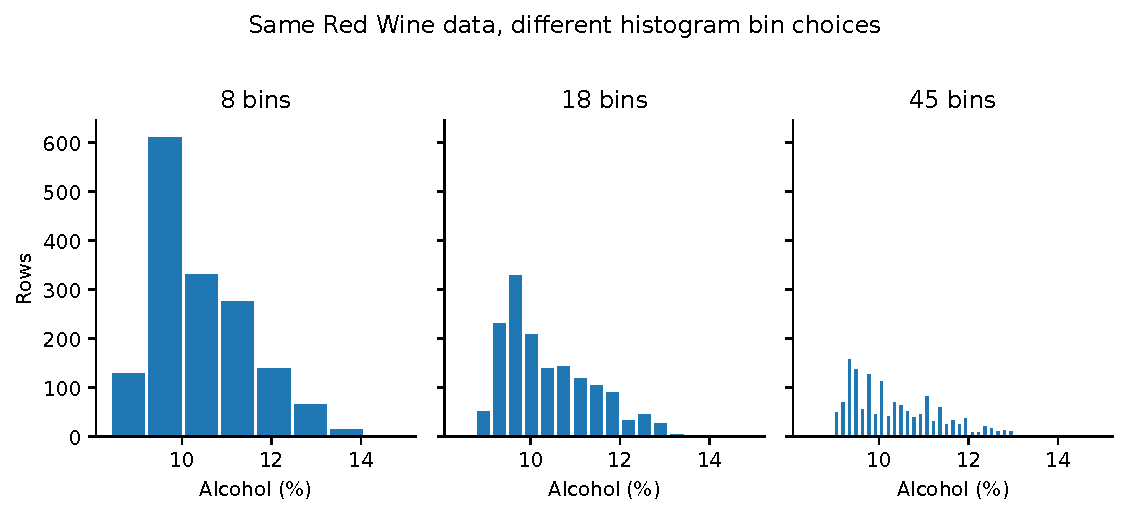
\includegraphics[width=0.91\linewidth]{figures/viz_histogram_bins.pdf}
\end{utpfig}

\section{Density, box, and violin-style views answer different questions}
A histogram or density estimate emphasises shape. A box plot emphasises median, quartiles, and outlier flags. A violin plot combines a density-like shape with a group comparison, but can suggest more precision than the sample supports when groups are small. Choose the representation that exposes the property the reader needs to compare.


\section{Box plots compare distributions compactly}
A box plot shows the median, quartiles, and potential outliers. It is effective for comparing several groups, but it hides detailed shape and sample-size differences unless additional context is provided.


\begin{utpfig}[Compact group comparison]{The same measurement can have overlapping but distinct group distributions. Box plots make medians and spread easy to compare, while the chapter's scatterplot will show within-group relationships.}{fig:viz-boxplot}
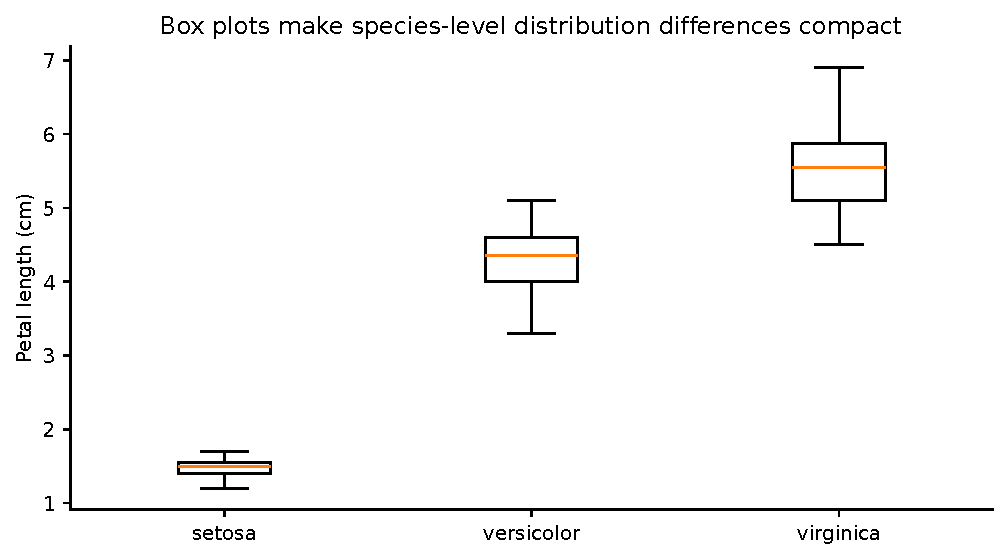
\includegraphics[width=0.77\linewidth]{figures/viz_boxplot_species.pdf}
\end{utpfig}


\section{Scatterplots are the default for two numeric variables}
A scatterplot can reveal linear or curved relationships, changing variance, distinct clusters, and influential points that one correlation coefficient cannot show.


\begin{utpfig}[Scatterplots reveal structure hidden by one coefficient]{Petal length and width have a strong overall relationship, but colour reveals three species-level groups and different local ranges.}{fig:viz-iris-scatter}
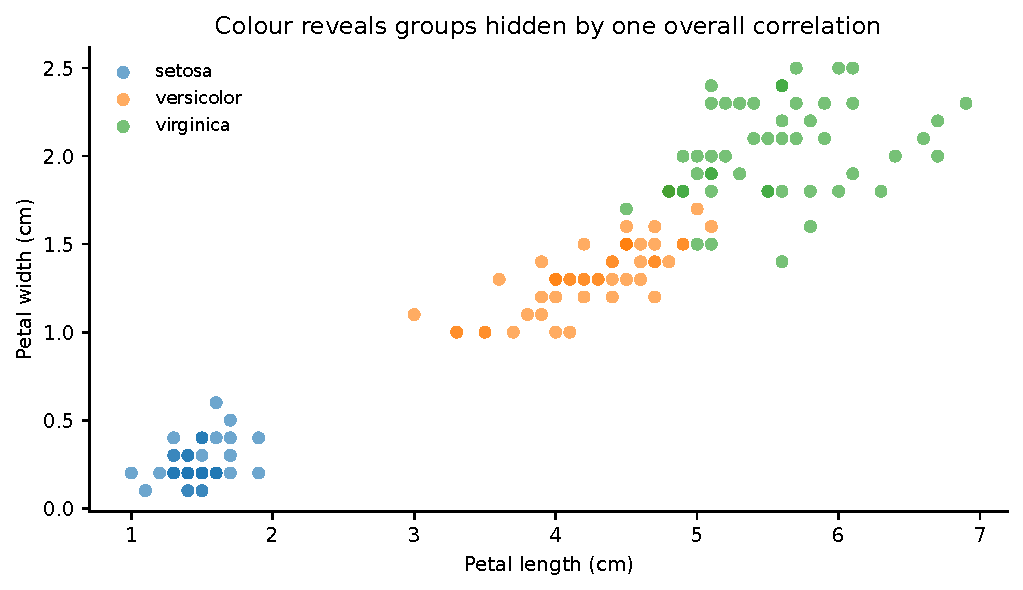
\includegraphics[width=0.76\linewidth]{figures/viz_iris_scatter.pdf}
\end{utpfig}

\section{Uncertainty should be visible when the claim is uncertain}
If a figure shows an estimated mean, fitted line, or model prediction, include an interval, error bar, distribution of resampled estimates, or another appropriate uncertainty display when possible. Showing only the point estimate can make an uncertain result appear exact.

\section{Design for comparison}
Good chart design places the values that need comparison on a common scale and close enough to compare. Small multiples are effective when several groups or time periods share the same axes. Sorting categories by a meaningful quantity can also reduce the mental work needed to find patterns.


\begin{pitfall}
Axis limits can exaggerate or conceal differences. Truncating a bar chart away from zero changes the perceived ratio of bar lengths; clipping a scatterplot can hide records that contradict the intended story. State and justify unusual scales.
\end{pitfall}

\section{A chart needs an evidence sentence}
Every figure should support a short interpretation that names the variables, describes the visible pattern, and separates observation from explanation.

\begin{workedexample}
Weak: ``The graph shows a relationship.''

Better: ``Petal length and petal width increase together, and the observations form visible species-level clusters. The plot establishes association and separation, not a biological causal mechanism.''
\end{workedexample}

\begin{keyidea}
Good visualisation reduces the distance between data and judgment. Remove decoration that does not encode information; keep labels, units, and context that make the evidence interpretable.
\end{keyidea}


\section{A visualisation review checklist}
Before publishing a chart, ask: Is the analytical question visible? Are units and population clear? Does the geometry match the variable type? Are scales honest and comparable? Is colour necessary and distinguishable? Are missing values or excluded groups acknowledged? Does the caption state the evidence rather than merely repeat the title? Could a reader misinterpret association as causation?


\begin{quickcheck}
\begin{enumerate}
  \item Why is position on a common axis easier to compare than area?
  \item What can a scatterplot reveal that correlation alone cannot?
  \item Why should histogram conclusions be checked across reasonable bin widths?
  \item What makes an interpretation sentence stronger than a chart title alone?
\end{enumerate}
\end{quickcheck}

\section{Worked visual design: red-wine quality}

The Red Wine Quality dataset contains 1,599 wines and an ordered quality score from 3 to 8. The outcome is numeric in storage but conceptually discrete and ordinal. That distinction affects chart design.

\begin{utpfig}[Alcohol content across ordered quality scores]{Boxplots preserve the discreteness of the quality score while showing a systematic shift in the alcohol distribution. The figure supports comparison without pretending that every one-unit quality change is exactly equivalent.}{fig:viz-redwine-alcohol}
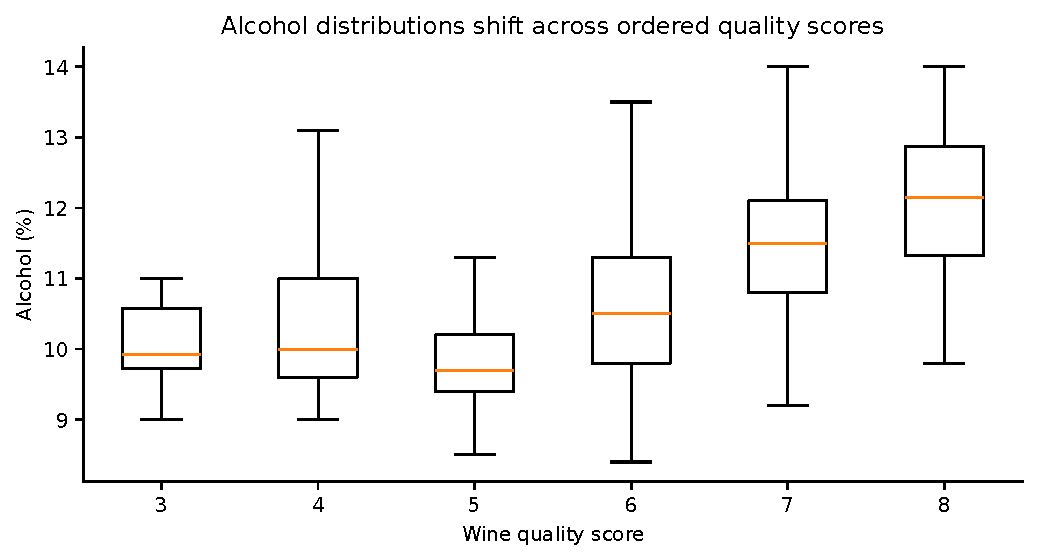
\includegraphics[width=0.82\linewidth]{figures/viz_wine_quality_alcohol.pdf}
\end{utpfig}

The correlation between alcohol and quality is about 0.48, but the boxplots communicate more: the quality groups overlap substantially and sample sizes are very unequal. Scores 5 and 6 dominate the dataset, whereas extreme scores are rare. A regression line alone would hide both facts.

\begin{keyidea}
The best chart is not the chart with the most aesthetics. It is the chart whose visual encoding makes the comparison required by the question easy and honest.
\end{keyidea}


\section{A second visual-design case: when two discrete dimensions interact}

The Bike Sharing hourly table contains two discrete coordinates that are easy to lose in a sequence of separate bar charts: hour of day and weekday. A heatmap uses position in two dimensions and colour for mean demand, allowing the reader to scan for recurring temporal structure.

\begin{utpfig}[Bike demand varies jointly by hour and weekday]{The heatmap makes morning/evening weekday peaks and broader weekend daytime use visible in one compact display. A one-dimensional average by hour would blur some of this structure.}{fig:viz-bike-heatmap}
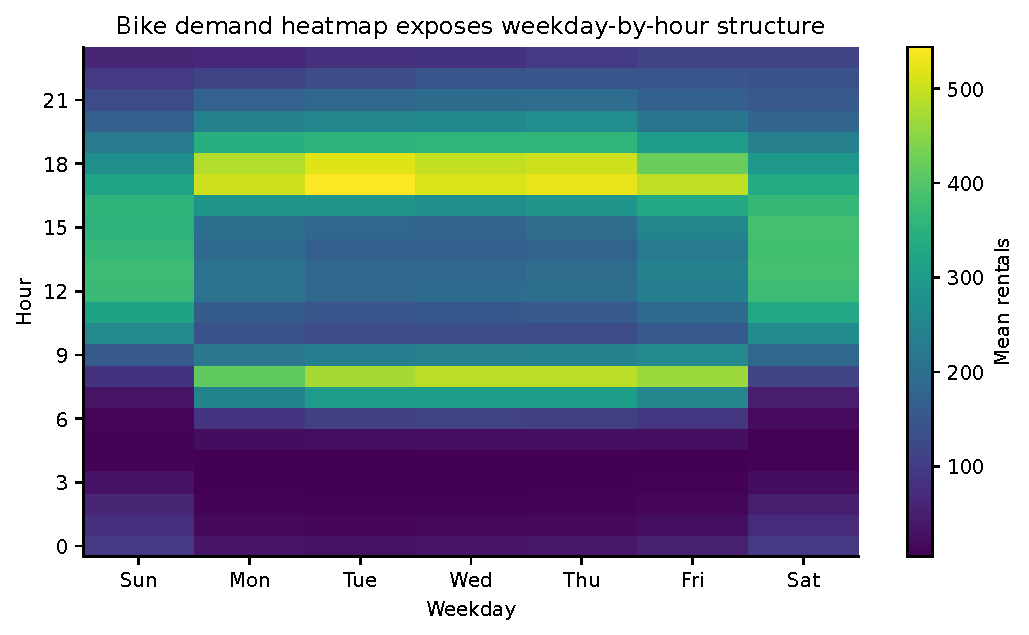
\includegraphics[width=0.80\linewidth]{figures/viz_bike_heatmap.pdf}
\end{utpfig}

This example also illustrates a design principle: aggregation should match the visual question. Each cell is a mean across many observed hours. The chart is therefore suitable for a recurring pattern, but not for showing day-to-day volatility, weather shocks, or uncertainty around each cell. A professional report should not ask one graphic to answer all of those questions simultaneously.

\labsection{5}{Design graphics that answer a question}{sec:lab05}

\begin{labproject}{Visual communication: turn analysis into evidence}
\textbf{Coverage.} Chapter~\ref{ch:visualization}.\\
\textbf{Goal.} You should be able to map analytical questions to chart forms, identify misleading encodings, write evidence-focused captions, and distinguish information revealed by raw and aggregated views.\\
\textbf{Datasets.} \texttt{red\_wine\_quality\_dataset.csv}; Bike Sharing hourly data are used for the extension.\\
\textbf{Scenario.} You are preparing figures for an analytical report. The objective is not decoration: each chart must answer a specific question, use an appropriate visual encoding, and make the intended comparison easy to see.

\textbf{Core design tasks.}
\begin{enumerate}
  \item \textbf{Distribution question.} Use a bar chart to show the frequency of the discrete wine-quality scores. Explain why a histogram is not the clearest default for this variable.
  \item \textbf{Group-comparison question.} Use side-by-side boxplots to compare alcohol content across quality scores. Support the figure with grouped numerical summaries.
  \item \textbf{Relationship question.} Use a scatterplot to examine volatile acidity and alcohol. Describe what can and cannot be inferred when neither variable is an outcome in the graphic.
  \item \textbf{Redesign by changing the question.} Create a second version of one figure that answers a genuinely different analytical question. Do not count changes in colour, font, or theme as a redesign.
  \item \textbf{Write analytical captions.} For each figure, state the data subset, visual encoding, main visible pattern, and one limitation or uncertainty.
  \item \textbf{Perform a visual integrity check.} Identify one choice that would exaggerate, hide, or confuse the pattern---for example, an inappropriate axis, unnecessary 3-D effect, excessive overplotting, or treating a discrete score as continuous without explanation.
\end{enumerate}

\begin{tryit}
\textbf{Extension---two-dimensional time structure.} Use \texttt{bike\_sharing\_dataset\_hour.csv} to create an hour-by-weekday heatmap of mean rentals. Explain what the heatmap reveals about commuting structure that a single hourly line cannot, and identify what variability is hidden by averaging.
\end{tryit}

\tcbbreak
\lstinputlisting[style=utpr]{all_experiments/lab05_visualization.R}
\begin{verification}
\textbf{Required evidence.} Submit a three-figure mini-report. Each figure must have a one-sentence question above it and a two-to-three sentence evidence caption below it. A reader should understand the analytical claim without seeing the R code.

\textbf{Professional standard.} Prefer the simplest chart that makes the required comparison accurately. Visual complexity is justified only when it reveals additional structure.
\end{verification}
\end{labproject}

